\chaplbl{Terminology}{s:terms}

The following terms will support the discussions and activities in the
rest of the training by giving us a common vocabulary to talk about
teaching and learning to teach.

\subsubsection{Educational Psychology}\label{educational-psychology}

\emph{Educational psychology} is the study of how people learn. It
touches on everything from the neuropsychology of perception and the
mechanisms of memory to the sociology of school systems and the
philosophical question of what we actually mean by ``learning'' (which
turns out to be pretty complicated once you start looking beyond the
standardized Western classroom). Within the broad scope of educational
psychology, two specific perspectives have primarily influenced Software
and Data Carpentry's lessons and teaching practices (and by extension,
this instructor training).

One perspective is \emph{cognitivism}, which treats learning as a
problem in neuropsychology. Cognitivists focus their attention on things
like pattern recognition, memory formation, and recall. It is good at
answering low-level questions, but generally ignores larger issues like,
``What do we mean by `learning'?'' and, ``Who gets to decide?''

Our other guiding perspective is
\emph{\href{https://en.wikipedia.org/wiki/Situated\_learning}{situated
learning}}, which focuses on the way that
\emph{\href{https://en.wikipedia.org/wiki/Legitimate\_peripheral\_participation}{legitimate
peripheral practice}} leads to people becoming members of a
\emph{\href{https://en.wikipedia.org/wiki/Community\_of\_practice}{community
of practice}}.

Unpacking those terms, the situated learning perspective focuses on the
transition from being a newcomer to being accepted as a peer by those
who already do the activity in question. Situated learning is directly
relevant to our learners, many of whom ease into scientific computing by
doing small tasks that experienced practitioners would regard as
straightforward, but who learn how to take on bigger and more novel
challenges both from what they do and from the feedback (and welcome) it
elicits. It is equally relevant to our instructors (i.e., you), who are
approaching evidence-based teaching in the same way.

Software and Data Carpentry aim to serve researchers who are exploring
data management and programming on their own (legitimate peripheral
practice) and make them aware of other people doing that work (simply by
attending the workshop) and the best practices and ideas of that
community of practice, thereby giving them a way to become members of
that community. Situated learning thus describes why we teach, and
recognizes that teaching and learning is necessarily rooted in a social
context. We then depend on the cognitivist perspective to drive
\emph{how} we teach the specific content associated with the community
of practice.

\begin{callout}{Other Perspectives}{callout:other-perspectives}

There are many other perspectives outside cognitivist theory---see
\href{http://www.learning-theories.com/}{this site} for summaries.
Besides cognitivism, those encountered most frequently include
\emph{behaviorism} (which treats education as stimulus/response
conditioning), \emph{constructivism} (which considers learning an active
process during which learners construct knowledge for themselves),
\emph{connectivism} (which emphasizes the social aspects of learning,
particularly those made possible by the Internet), and
\emph{connectionism}, a cognitivist theory that explains learning as
creating connections between concepts. And yes, it would help if their
names were less similar\ldots{}
\end{callout}

\subsubsection{Instructional Design}\label{instructional-design}

Educational psychology does not tell us how to teach on its own because
it under-constrains the problem: in real life, several different
teaching methods might be consistent with what we currently know about
how learning works. We therefore have to try those methods in the class,
with actual learners, in order to find out how well they balance the
different forces in play. This is called \emph{instructional design}
(ID); if educational psychology is the science, ID is the engineering.

\subsubsection{Pedagogical Content
Knowledge}\label{pedagogical-content-knowledge}

In the end, effective teaching often depends on what the teacher knows.
The things teachers know can be divided into:

\begin{itemize}
\item
  \emph{content knowledge}, such as the ``what'' of programming;
\item
  \emph{general pedagogical knowledge}, i.e., an understanding of the
  psychology of learning; and
\item
  the \emph{pedagogical content knowledge} (PCK) that connects the two.
  PCK is things like what examples to use when teaching how parameters
  are passed to a function, or what misconceptions about wildcard
  expansion are most common.
\end{itemize}

\begin{figure}[htbp]
\centering
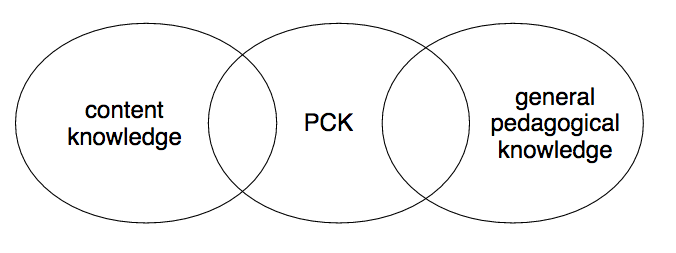
\includegraphics{../fig/pck.svg}
\caption{Pedagogical Content Knowledge}
\end{figure}

This training course focuses on general pedagogical knowledge through
the two major categories (educational psychology and instructional
design) described above. It assumes you know as much as you need to
about basic programming (our content knowledge).

When it comes to PCK, we will see later \secref{sec:practices} some
of the PCK of the Software and Data Carpentry communities at
work. Within Software Carpentry, we are also trying to support the
curation of PCK by including an instructor's guide with each lesson
that describes particular teaching techniques for that lesson's
content.

Finally, this training includes times for discussion, observation, and
feedback, precisely so that participants are able to share their PCK
with each other over the course of the next two days.

\begin{callout}{Examples of PCK}{callout:examples-of-pck}

\begin{itemize}
\item
  Gelman and Nolan's
  \textit{Teaching   Statistics: A Bag of Tricks} \cite{bib:gelman-nolan-stats-tricks}
  is full of PCK for teaching introductory statistics.
\item
  The \href{http://csteachingtips.org/}{CS Teaching Tips} site is
  gathering similar ideas for computing.
\end{itemize}
\end{callout}

\subsection{Myths and Pseudoscience}\label{myths-and-pseudoscience}

One
\href{https://en.wikipedia.org/wiki/Learning\_styles\#Learning\_modalities}{well-known
scheme} characterizes learners as visual, auditory, or kinesthetic
according to whether they like to see things, hear things, or do things.
This scheme is easy to understand, but as de Bruyckere and colleagues
point out in
\textit{Urban Myths About Learning and Education} \cite{bib:debruyckere-urban-myths},
it is almost certainly false.
Unfortunately, that hasn't stopped a large number of companies from
marketing products based on it to parents and school boards.

This is not the only myth to plague education. The learning pyramid that
shows we remember 10\% of what we read, 20\% of what we hear, and so on?
Myth.
The idea that ``brain games'' can improve our intelligence, or at least
slow its decline in old age?
Also a myth, as are the claims that the Internet is making us dumber or that
young people read less than they used to.

Computing education has its own myths. Mark Guzdial's
``Top 10 Myths About Teaching Computer Science'' \cite{bib:guzdial-top10} are:

The lack of women in Computer Science is just like all the other STEM
fields.

To get more women in CS, we need more female CS faculty.

A good CS teacher is a good lecturer.

Clickers and the like are an add-on for a good teacher.

Student evaluations are the best way to evaluate teaching.

Good teachers personalize education for students' learning styles.

High schools just can't teach CS well, so they shouldn't do it at all.

The real problem is to get more CS curriculum out into the hands of
teachers.

All I need to do to be a good CS teacher is model good software
development practice, because my job is to produce excellent software
engineers.

Some people are just born to program.

The last of these---the idea that there is a ``geek gene''---is as
pervasive as it is damaging. Elizabeth Patitsas and others have shown
that, contrary to a widely-held belief,
grades in computing classes are \emph{not} bimodal \cite{bib:patitsas-cs-grades},
i.e., there isn't one group that gets
it and another that doesn't. Many of the participants in our workshops
have advanced degrees in intellectually demanding subjects, but have
convinced themselves that they just don't have what it takes to be
programmers. If all we do is dispel that belief, we will have done them
a service.

\begin{callout}{Key Readings}{callout:key-readings}

An excellent overview of research results in education and learning is
Ambrose et al's
\textit{How Learning Works} \cite{bib:ambrose-hlw} (which is also an excellent example of what secondary
literature ought to look like).  Green's
\textit{Building a Better Teacher} \cite{bib:greene-babt} is lighter but no less informative: it explores why
educational reforms in the past 50 years have mostly missed the mark,
and what we should be doing instead. The ultra-short summary
Deans for Impact report \cite{bib:deans-for-impact} contains useful, practical insights, and is
required reading for this training.

Pieces focusing specifically on computer science education include
Guzdial's
``Why Programming is Hard to Teach'' \cite{bib:guzdial-hard} and
``Top 10 Myths About Teaching Computer Science'' \cite{bib:guzdial-top10},
and Porter et al's ``Success in Introductory Programming: What Works?'' \cite{bib:porter-what-works},
all of which you should read before starting this class.
\end{callout}

\begin{discussion}{Three Kinds of Knowledge}{disc:three-kinds-of-knowledge}

Think of a memorable moment from a class you took or taught. Describe
it, and explain how the instructor used domain knowledge, general
pedagogical knowledge, and pedagogical content knowledge to create that
moment.
\end{discussion}

\begin{discussion}{Bottom Up or Top Down?}{disc:bottom-up-or-top-down}

How would you describe the way you learned what you already know about
using computers in research: bottom up, top down, or a mix of both? Is
that how you prefer to learn?
\end{discussion}
